\documentclass{standalone}

\usepackage{tikz}
\usepackage{circuitikz}

\tikzset{block/.style = {draw, fill=white, very thick, rectangle, minimum height=1cm, minimum width=2cm},
         lblock/.style={draw,fill=white,very thick, rectangle, minimum height=3cm, minimum width=1cm},
         sum/.style= {draw, fill=white, very thick, circle, node distance=0.5cm}}

         
\begin{document}
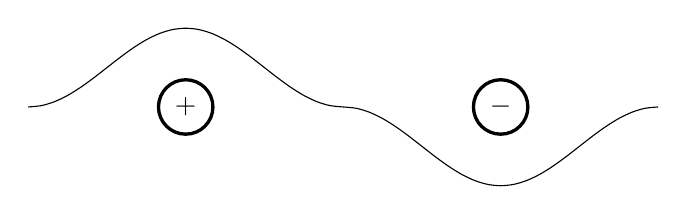
\begin{tikzpicture}[scale=2]
    \node[sum](o1)at(0,0){$+$};
    \draw[-]plot[smooth, domain=-1:1](\x,{-0.25*cos(180*(\x)-pi r)+0.25});
    
    \node[sum](o2)at(2,0){$-$};
    \draw[-]plot[smooth, domain=1:3](\x,{0.25*cos(180*(\x-2)-pi r)-0.25});
\end{tikzpicture}
\end{document}